\subsection{Loss and accuracy vs. epochs}

As anticipated, Fig. \ref{fig:epochs} allows to visualize the trends of training and validation loss and accuracy of the two models during the training phase relatively to the epoch number. 
\\ Observe that, while the metrics relative to the training set smoothly decrease and increase respectively, the ones relative to the validation set show a more erratic behavior. It is probably due to the composition of the dataset, which is possibly noisy and unbalanced, and to the fact that the validation set is not very large: this is supported by the fact that this phenomenon occurrs for both models, even though model 1 is slightly less affected by it, probably because of its structure and of the Nesterov momentum in the Nadam optimizer.
\\Anyway, the early stopping callback does its job of preventing overfitting: the best weights are achieved at the 22nd epoch for model 0 and at the 26th for model 1, and those are the ones that are used for the evaluation phase.

\begin{figure}[htbp]
    \centering
    \subfloat[Model 0.]{
        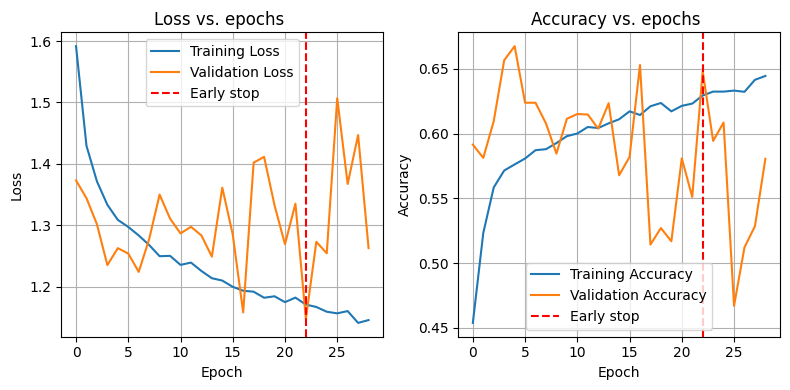
\includegraphics[width=0.7\textwidth]{figures/images/epochs_m0.png}
        \label{fig:epochs_m0}
    }
    \\
    \subfloat[Model 1.]{
        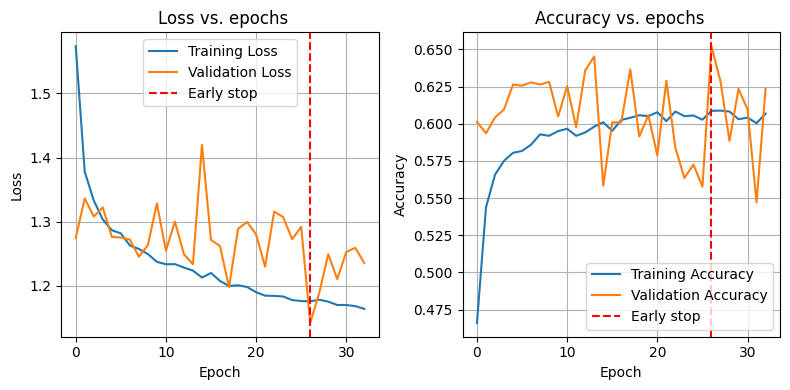
\includegraphics[width=0.7\textwidth]{figures/images/epochs_m1.png}
        \label{fig:epochs_m1}
    }
    \caption{Graph of loss and accuracy of the two models during the training phase, highlighting the point of early stopping.}
    \label{fig:epochs}
\end{figure}